\chapter{配置ROS路由器}
%\label{cha:ros}

\section{ROS介绍}
MikroTik RouterOS\cite{ros}是一种路由操作系统,并通过该软件将标准的PC电脑变成专业路由器,在
软件的开发和应用上不断的更新和发展,软件经历了多次更新和改进,使其功能在不断增强和完善。特
别在无线、认证、策略路由、带宽控制和防火墙过滤等功能上有着非常突出的功能,其极高的性价比,
受到许多网络人士的青睐。RouterOS在具备现有路由系统的大部分功能,能针对网吧、企业、小型ISP接
入商、社区等网络设备的接入,基于标准的x86构架的PC。一台586PC机就可以实现路由功能,提高硬件
性能同样也能提高网络的访问速度和吞吐量。完全是一套低成本,高性能的路由器系统。

\section{基本功能介绍}

\begin{itemize}
\item 完整的防火墙设置功能,隧道协议和Ipsec功能;
\item 多线路支持(负载均衡、双线路由、静态路由、策略路由);
\item P2P传输过滤过滤功能高效的VRRP(虚拟路由冗余协议)强大的QoS功能带宽流量控制;
\item 网桥功能并支持STP;
\item 支持WEP的超高速802.11a/b/g无线协议;WDS和虚拟AP特征;
\item 支持即插即用UPNP;
\item RIP, OSPF, BGP路由控制协议;
\item 提供1G以太网接口;
\item 同步支持V.35, X.21, T1/E1系列;
\item 实现Hotspot的web网络认证管理功能;
\item 支持PPPoE和PPTP客户端与服务器;
\item Radius计费功能;IP电话功能(H323);
\item 远程WinBox和Web管理;
\item telnet/ssh/serial管理控制台;
\item 实时配置和监控;
\end{itemize}

\section{硬件准备}

\begin{enumerate}
\item 首先下载软路由的ghost硬盘版,如果没有,从\url{http://www.nbwq.com/download/ros297.rar}下载
\item 释放后,ghost至一个小硬盘($20G$以下),注意,是整盘GHOST而不是分区。
\item 将该硬盘挂在要做路由电脑上,注意必须接在第一个IDE并且是主硬盘接口。插上一张网卡,这是接内网的LAN。开机。
\end{enumerate}

\section{软件设置}

\begin{enumerate}
\item 开机,出现登陆提示。用户:admin 密码:空
\item 输入setup再按两次A
\item 在ether1后面输入你的内网IP,如:192.168.0.254/24 (这里/24是24位掩码与255.255.255.0一
  样)
\item 输入完ip后,按两次x退出,现在可以可以ping通192.168.0.254了,也可用winbox在图形界面下
  访问路由了。
\item 关机,插上另一张网卡,这个是接外网的,即WAN,现在可以去掉软路由电脑的显示器和键盘了。
\item 开机,运行winbox以admin身份登陆
\item 添加外网网卡。在ip—address里按+,address输入你的外网ip和掩码位,比
  如218.56.37.11/29。network和BROADCAST不填,INTERFACE里选择ethr2
\item 增加外网网关。ip-routes按+,Destination用默认的0.0.0.0/0 ,Gateway输入外网网关,比
  如218.56.37.10
\item 实现NAT转发:IP-FIREWALL在NAT里点+,在ACTION里选masquerade
\item 现在该路由已经做好雏形,可以正常上网了。
\end{enumerate}

\subsection{Router OS路由器各种登录方式}

Mikrotik routerOS 内能通过运程配置各种参数, 包括 Telnet,SSH,winbox 和
Webbox。

\subsubsection{winbox运行界面}

\begin{figure}[h]
  \centering
  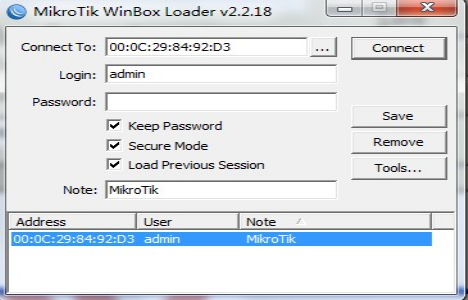
\includegraphics[width=.7\textwidth]{pic/winbox.png}
  \caption{winbox登录界面}
  \label{fig:winbox} 
\end{figure}

MAC-telnet是在路由器没有IP地址的情况下或者配置防火墙参数后无法连接,通过路由器网卡MAC地址登
陆的方式远程连接到路由器, MAC-telnet仅能使用在来自同一个广播域中(因此在网络中不能有路由的存
在),路由器的网卡应该被启用。注意,在winbox中通过MAC地址连接路由器的功能,并内置了探测工具。
这样在管理员忘记或复位了路由器后,同样可以通过 MAC 登录到 routerOS 上,进行图形界面操作

\subsection{winbox 图形操作界面}

Winbox 控制台适用于 mikrotik routerOS 的管理和配置,使用图形管理和配置,使用它型管理接
口(GUI)。通过连接到 mikrotik 路由器的 HTTP(TCP 80 端口)欢迎界面下载 Winbox.exe 可行文件,下
载并保存在你的 windows 中,之后直接在你windows 电脑上运行 Winbox.exe 文件。

\begin{itemize}
\item
\includegraphics{pic/winbox1.png}搜索和显示 MNDP (mikrotik Neighbor discovery
  protocol) 或 CDP(cisco discovery protocol)设备,可以通过该功能键搜索同一子网
  内 mikrotik 和 cisco设备,并能通过 MAC 地址登陆到 mikrotik routerOS 进行操作。
\item 
\includegraphics{pic/winbox2.png}通过指定的 IP 地址(默认端口为 80,不许特别指定,如果你
  修改了端口需要对具体访问端口做自定)或 MAC 地址(如果路由器在同一子网内)登陆路由器。
\item 
\includegraphics{pic/winbox3.png}保存当前连接列表(当需要运行它们时,只需双击)。
\item 
\includegraphics{pic/winbox4.png}删除从列表中选择的项目。
\item 
\includegraphics{pic/winbox5.png}所有列表中的项目,清除在本地的缓存,从 Winbox 文件导入
  地址或导出为 Winbox 文件。
\item 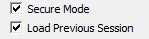
\includegraphics{pic/winbox6.png}Secure mode (安全模式):提供保密并
  在 Winbox 和routerOS 之间使用 TLS(transport layer security)协议; Keep password(保存密码):保
  存密码到本地磁盘的文本文件中。
\end{itemize}

\subsection{MAC 层访问(telnet 与 winbox)}

通过MAC地址进行链接是用来访问没有设置IP地址的routerOS路由设备,这种连接类似于IP地址
连接,通过MAC地址仅在限于2台mikrotik routerOS路由器之间进行, 操作路径: \verb|/tool/mac-server|。

\subsection{常用命令信息}
在任何操作目录使用‘?’都可用获在当前目录中的命令信息。
\begin{multicols}{2}
  \begin{description}
  \item[log/] --- 系统日志
  \item[Quit]---退出控制台
  \item[Radius/]---客户端设置
  \item[Certificate/]---授权管理
  \item[Special-login/]---特殊登陆用户
  \item[Ping-ping] ---命令
  \item[Setup]---基本的系统设置
  \item[Interface/]---接口配置
  \item[Password]---修改密码
  \item[Undo]---撤销以前操作
  \item[Port/]---串口控制
  \item[User/]---用户管理
  \item[System/]---系统信息和应用程序
  \item[Ip/-ip] ---选项
  \item[Tools/]---工具
  \item[Routing]---各种路由协议设置
  \item[..]---回到根目录
  \item[Address/]---地址管理
  \item[Route/]---路由管理
  \item[Firewall/]---防火墙管理
  \item[DHCP-client]---DHCP 客户端设置
  \item[DHCP-serner/]---DHCP 服务设置
  \item[Hotspot/-hotspot] ---管理
  \item[Pool-ip] ---地址池
  \end{description}
\end{multicols}

一个指令或一个变量参数不需要完整的输入, 如是含糊不清的指令或变量参数需要完整的输输
入 interface 时,你只要输入 in 或 int,需要显示完整的指令可以使用[tab]键通过指令的组合,可以在
当前的目录执行在不同目录操作

\section{配置步骤}

基本配置完成以后需要配置我们需要的ROS,对于酒店的特殊需求,我自己配置了一份ROS配置文件,
这样的好处是可以批量配置路由器,不用每次手工配置,步骤如下:
\begin{enumerate}
\item 使用winbox登录ROS,输入用户名密码。
\item 鼠标点击New Terminal,出现一个终端,复制配置文件backup.rsc(见附录~\ref{sec:ros-script})。
\item 鼠标放到终端上点击粘贴。
\item 配置成功。
\item 配置文件详见附录~\ref{sec:ros-script}。
\end{enumerate}




%%% Local Variables: 
%%% mode: latex
%%% TeX-master: "../thesis"
%%% End: 
